\documentclass[margin,line]{CV}

\usepackage{graphicx}
\usepackage{wrapfig}
\usepackage{ifthen}
\usepackage{url}

\newboolean{foreign}
\setboolean{foreign}{false}

\begin{document}
\name{\Large Fokin Alexander}
\begin{resume}

%\begin{wrapfigure}{r}{2cm}
%    \vspace{-20pt}
%    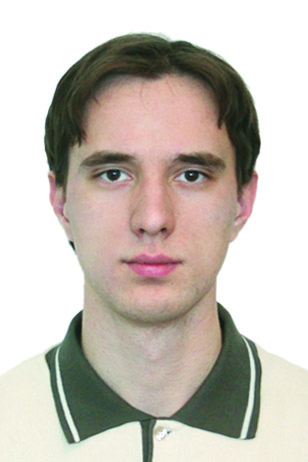
\includegraphics[width=2cm]{photo.jpg}
%    \vspace{-20pt}
%\end{wrapfigure}

    \section{\mysidestyle Contact\\Information}
    Current Location: Los Angeles, United States \\
    \\
    Mobile: 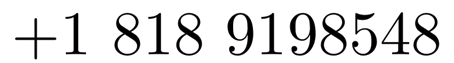
\includegraphics[height=0.35cm]{phone-us.png} \\ 
    E-mail: apfokin@gmail.com \\
    \\

    \section{\mysidestyle Professional\\Experience}
    \textbf{Network Optix, Inc.} \vspace{2mm}\\\vspace{1mm}%
    \textsl{Senior Software Engineer} \hfill \textbf{October 2011 - present}\\
    I'm currently working on HD Witness, an Enterprise Video Management System (VMS). 
    
    For the initial release I have almost single-handedly implemented the client application that was very well received in the industry. Various sources have described HD Witness as the most visually appealing and user-friendly VMS on the market, which has helped the company to gain a competitive edge.
    
    Currently my main responsibilities include ensuring UI and UX performance and consistency of our desktop and mobile clients, management of the front-end development team, design of public APIs and development of generic C++ libraries that are used internally.

    
	\textbf{Combild} \vspace{2mm}\\\vspace{1mm}%
	\textsl{Software Development Lead, Co-founder} \hfill \textbf{June 2010 - December 2011}\\
    Combild was stated to create a program complex for IT infrastructure management that would target small companies and IT outsourcers. At the moment all other solutions on the market were either too bulky and hard to maintain, or were not suitable for the business model of IT outsourcers. Frustrated with the state of things, we have decided to roll out our own product.
    
    At Combild I have laid out the overall product architecture, was working with customers to prioritize and clarify the features and was managing a small development team.
    
    %After a year of development we have secured our first customers, but at that point the cash inflow we had wasn't sufficient to cover our expenses. Unable to secure the funding, we had to close the project.

    
    \textbf{Select LTD} \vspace{2mm}\\\vspace{1mm}%
    \textsl{Software Engineer} \hfill \textbf{July 2009 - September 2011}\\
    I was leading the development of SmartDec, a native code decompiler. I have laid out the architecture of the decompiler and have implemented several frontend and backend plugins, including support for different x86 and PIC assembly input formats. I was also responsible for devising novel algorithms that would improve the quality of the decompiled code and would allow for reconstruction of C++-specific constructs. This effort has lead to several publications on international conferences on reverse engineering. Detailed description of the decompiler is available at \url{http://decompilation.info}.
    
    As one of the side projects at Select LTD I have implemented a form recognition toolkit that was subsequently used in some of the Moscow schools for test checking. I have also participated in the development of business processes and supporting infrastructure for this project. Detailed description is available at \url{http://elric.ru/wordpress/projects/form-recognition-toolkit/}. 

    I was also doing some work on \url{http://mathege.ru}, a portal for national mathematics exam in Russia. I did both frontend and backend development and have implemented a \LaTeX to html converter that was used for importing problems into the system.

    
    \textbf{Institute for System Programming of the Russian Academy of Sciences} \vspace{2mm}\\\vspace{1mm}%
    \textsl{Software Engineer} \hfill \textbf{September 2007 - September 2008}\\
    At ISPRAS I was working in a team developing a framework for dynamic analysis of binary code. Using C++ metaprogramming techniques I have implemented a disassembler for MIPS64 architecture that outperformed all other disassemblers for this architecture known to our team.

    \pagebreak    
    
    \textbf{Intel Research Lab at the Moscow State University} \vspace{2mm}\\\vspace{1mm}%
    \textsl{Software Engineer} \hfill \textbf{February 2007 - April 2008}\\
    At Intel Lab I was learning computer vision algorithms and have implemented a panorama stitching application. Description is available at \url{https://code.google.com/p/prec/}.

    As a side project I have implemented Ruby bindings for Intel's Integrated Performance Primitives library. Description is available at \url{https://code.google.com/p/ipp4r/}.
    
    
	\textbf{Personal Projects} \vspace{2mm}\\\vspace{1mm}%
    I am an avid programmer and I enjoy writing code in my free time. Throughout the years I have done some work as a freelance programmer and has finished several personal projects. For more information check out my google code page (\url{https://code.google.com/u/100177180062339664882/}) and my personal website (\url{http://elric.ru/wordpress/projects}).
   
    
    \section{\mysidestyle Education}
    \textbf{Faculty of Computational Mathematics and Cybernetics, Moscow State University}, Moscow, Russia \vspace{2mm}\\\vspace{1mm}%
    \textsl{\ifthenelse{\boolean{foreign}}{Bachelor's}{Specialist} degree in Applied Mathematics and Computer Science} \hfill \textbf{September 2004 - July 2009}\vspace{1mm}\\
    Advisor: Professor Chernov Alexander \\
    Thesis: Reconstruction of Class Hierarchies for Decompilation of C++ Programs \\
    I have graduated with high honors. Diploma GPA is 5.0 out of 5.0.

    \textbf{Graduate School of Science and Engineering, Chuo University}, Tokyo, Japan \vspace{2mm}\\\vspace{1mm}%
    \textsl{Full-time non-degree student} \hfill \textbf{September 2008 - March 2009}\vspace{1mm}\\
    Advisor: Professor Mitsunori Makino \\
	I was studying Japanese, working on algorithms for real-time ray tracing and have implemented a real-time ray tracer for use with CAVE automatic virtual environment.

%    \section{\mysidestyle Research\\Interests}
%    Image-based modeling and rendering, 3d reconstruction.
%    Ray tracing and global illumination, especially in real time.
%    Software reverse engineering, binary translation, decompilation.

%    \section{\mysidestyle Research\\Experience}
%    \textbf{Select LTD} \vspace{2mm}\\\vspace{1mm}%
%    \hfill \textbf{October 2010 - September 2011}\\
%    I continued my work on C++ decompilation at Select LTD. 

%    \textbf{Institute for System Programming of the Russian Academy of Sciences} \vspace{2mm}\\\vspace{1mm}%
%    \hfill \textbf{July 2008 - September 2010}\\
%    I was doing research on decompilation of C++ programs.


    \section{\mysidestyle Publications}
    A. Fokin, E. Derevenetc, A. Chernov and K. Troshina. ``SmartDec: Approaching C++ Decompilation'',
	in proceedings of the \textsl{18th Working Conference on Reverse Engineering}, pp. 347-356, 2011.
	
	A. Fokin, K. Troshina and A. Chernov. ``Reconstruction of Class Hierarchies for Decompilation of C++ Programs'',
    in proceedings of the \textsl{14th European Conference on Software Maintenance and Reengineering}, pp. 249-252, 2010.

    K. Troshina, A. Chernov and A. Fokin. ``Profile-Based Type Reconstruction for Decompilation'',
    in proceedings of the \textsl{17th International Conference on Program Comprehension}, pp. 263-267, 2009.

    \pagebreak    
    
    \section{\mysidestyle Honours, \\Awards and \\Test Scores}
    TOEFL iBT, 111/120, Moscow, 2010.                                                               \vspace{1mm}\\%
    M.V. Lomonosov Scholarship for Academic Excellence, Moscow, 2006-2009.                          \vspace{1mm}\\%
    8th Moscow Collegiate Programming Contest, 9th place, Moscow, 2006.                             \vspace{1mm}\\%
    7th Moscow Collegiate Programming Contest, 11th place, Moscow, 2005.                            \vspace{1mm}\\%
    Unified State Exam in Mathematics, 100/100 (nationwide top), Izhevsk, 2004.                     \vspace{1mm}\\%

    \section{\mysidestyle Related\\Skills}
	Experience managing a small development team. \\
    Substantial experience with C++ and Java. \\
	Deep understanding of the underlying principles of modern C++ libraries and frameworks such as Qt and boost. \\
    A lot of experience writing cross-platform C++ code. \\
    Considerable experience with multithreading in C++ and Java. \\
    Knowledge of modern realtime rendering techniques and APIs. \\
    Experience with Delphi, x86 Assembly, Linux shell scripting, SQL. \\
    Some experience with C\#, Matlab, Perl and Python. \\


    \section{\mysidestyle Languages}
    Russian: native \\
    English: fluent \\
    Japanese: intermediate


    \section{\mysidestyle References}
    {\sl Available upon request.}

\end{resume}
\end{document}



















